% vim: spelllang=en_au
\documentclass[a4paper]{article}

\usepackage{geometry}
\usepackage{amsmath}
\usepackage{enumerate}
\usepackage{amssymb}
\usepackage{amsthm}
\usepackage{hyperref}
\usepackage{minted}
% \usepackage[symbol]{footmisc}
\usepackage{tikz}
\usetikzlibrary{automata}
\usetikzlibrary{positioning,arrows.meta,calc}
\usetikzlibrary{angles,intersections,quotes,arrows.meta}


\DeclareMathOperator{\lcm}{lcm}

\author{Kait Lam \\ \small \texttt{45294583} \\ \small {T02}}
\title{\textsc{Math3306} --- Assignment 1 (Submission)}
\date{16 August 2024}

\begin{document}

\maketitle


\section*{Question 1}
\subsection*{Question 1(a)}
\begin{center}
  \textit{Must a language over a single-letter alphabet be regular?}
\end{center}
Of course not.
Even with only a single letter, it is sufficiently powerful to represent any set of natural numbers.
Define
\begin{align*}
  L = \{w \in \{\star\}^* ~|~ \ell(w) = \langle M, x \rangle \text{ and } \texttt{TM}_M\text{ halts on input }x\}.
\end{align*}
That is, the language of encoded pairs of Turing machine number and input, such that the Turing machine halts on the given
input.
This is simply encoded within our single-letter alphabet as unary.
Were $L$ regular (that is, recognisable by a finite state automaton), this would easily decide the Halting problem,
contradicting the known undecidability of this problem.

% More generally, by way of encoding with prime factorisation and G\"odel numbering,
% any  can be represented as unary in a single-letter alphabet

% Assume, with the intent of contradiction, that $L$ is regular.
% It may be irregular.
% Consider the language
% \begin{align*}
%    L = \{ w \in \{\star\}^* ~|~ \ell(w)\text{ is prime}\}.
% \end{align*}
% Assume, with the intent of contradiction, that $L$ is regular and so the pumping lemma applies.
% By pumping, there exists $p_L > 1$ such that for all $w \in L$, 
% if $\ell(w) > p_L$, then there exists $x, y, z$ such that $w = xyz$ and 
% \begin{enumerate}[(i)]
%   \item $\ell(y) \ge 1$,
%   \item $\ell(xy)  < p_L$, and
%   \item $\forall n \ge 0, xy^nz \in L$.
% \end{enumerate}
% By property (iii), we can construct a word with non-prime length and assert it must be in $L$.
% To wit, the string
%   $xy^{2(\ell(x)+\ell(z))+1}z$.
% Observe,
% \begin{align*}
%   \ell(xy^{2(\ell(x)+\ell(z)+1)}z) &= \ell(x) + (2\ell(x) + 2\ell(z) + 1)\cdot \ell(y) + \ell(z) \\
%   &= 2(\ell(x) + \ell(z))\cdot(\ell(y) + 1)
% \end{align*}
% which is a non-prime length with factors $\ell(x) + \ell(z)$ and $\ell(y) + 1$.
% The pumping lemma claims this word is in $L$ which contradicts its original definition.
%
% As some technicalities,
% we note that due to infinitude of primes, we can obtain at least one $w \in L$ such that $\ell(w) > p_L$, in order to build our composite number.
% Also note that due to (i), $\ell(y) + 1 \ge 2$ and, due to (ii) and $\ell(xyz) > p_L$, $\ell(z) \ge 1$.
%
%
% x + n y + z
% x + 
% (2x + 2z) (y + 1) = 2xy + 2x + 2zy + 2z

% x + z + (2x + 2z) * y = x + z + 2xy + 2zy

\subsection*{Question 2(a)}
\begin{center}
  \textit{Recognise $L = \{0^{2n}~|~ n \ge 0\}$ with a Turing machine.}
\end{center}
We will write a recursive algorithm:
\begin{enumerate}[(1)]
  \setlength{\itemsep}{0pt}
  \item If the string is empty, accept.
  \item Otherwise, divide the input unary number by two, by
    \begin{enumerate}
      \item moving right and clearing every second space until the end of the string, then
      \item moving left and compressing the string, collapsing all cleared spaces.
    \end{enumerate}
  \item Go to (1).
\end{enumerate}
The division algorithm implicitly ensures that the number is divisible by two, otherwise it will halt
due to missing transitions.

\begin{figure}[h]
  \begin{center}
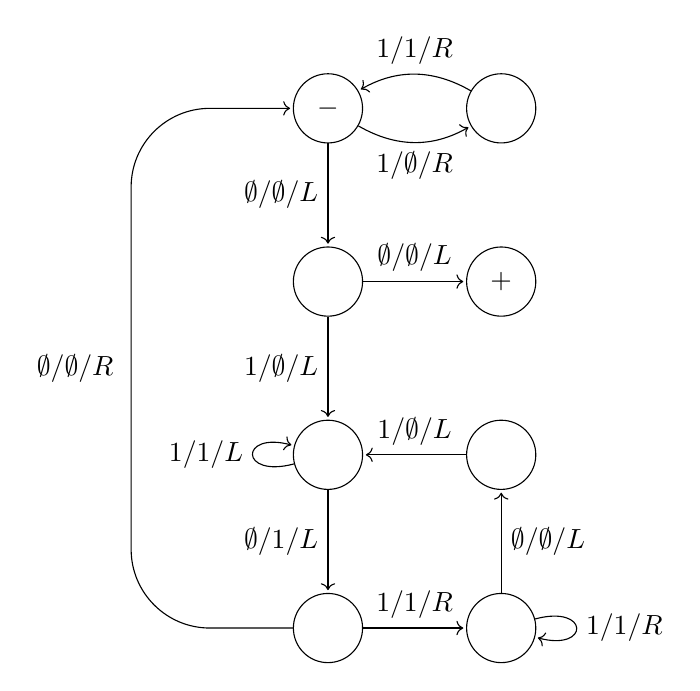
\begin{tikzpicture}[shorten >=1pt,node distance=2.2cm,on grid,auto] 

  \tikzset{
    rc/.style={rounded corners=2mm},
  }

   \node[state] (q0)   {$-$}; 
   \node[state] (first) [right=of q0] {};
   \path[->] (q0) edge [bend right] node [swap]{$1/\emptyset/R$} (first);
   % \node[state] (second) [right=of first] {};
   \path[->] (first) edge [bend right] node [swap]{$1/1/R$} (q0);

   \node[state] (base) [below=of q0] {};
   \path[->] (q0) edge node[swap] {$\emptyset/\emptyset/L$} (base);
   \node[state] (accept) [right=of base] {$+$};
   \path[->] (base) edge node {$\emptyset/\emptyset/L$} (accept);

   \node[state] (shift) [below=of base] {};
   \path[->] (base) edge node [swap]{$1/\emptyset/L$} (shift);
   \path[->] (shift) edge [loop left] node {$1/1/L$} (shift);

   \node[state] (shiftend) [below=of shift] {};
   \path[->] (shift) edge node [swap]{$\emptyset/1/L$} (shiftend);
   \node[state] (again) [right=of shiftend] {};
   \path[->] (shiftend) edge node {$1/1/R$} (again);
   \path[->] (again) edge [loop right] node {$1/1/R$} (again);
   \node[state] (restart) [above=of again] {};
   \path[->] (again) edge  node [swap]{$\emptyset/\emptyset/L$} (restart);
   \path[->] (restart) edge  node [swap]{$1/\emptyset/L$} (shift);

   \draw [->,rounded corners=1cm](shiftend) to
   ($(shiftend)+(-2.5, 0)$) to   node[xshift=-0.1cm]{$\emptyset/\emptyset/R$}($(q0)+(-2.5,0)$) to  (q0);
   

   

  %  \node[state] (qhash1) [above right=of q0] {}; 
  %  \path[->] (q0) edge node [swap]{$\#/\#/\mathrm R$} (qhash1);
  %  \node[state] (qhash2) [right=of qhash1] {$+$};
  %  \path[->] (qhash1) edge node {$\emptyset/\emptyset/\mathrm R$} (qhash2);
  %
  %  % ZEROS
  %
  %  \node[state] (qzero1) [below left=of q0]{$\rightarrow$};
  %  \path[->] (q0) edge node [swap]{$0/\emptyset/\mathrm R$} (qzero1);
  %  \path[->] (qzero1) edge [loop left] node {$[01]/[01]/\mathrm R$} (qzero1);
  %
  %
  %  \node[state] (qzerocheck) [below =of qzero1]{};
  %  \path[->] (qzero1) edge  node [swap]{$\#/\#/\mathrm R$} (qzerocheck);
  %
  %  \node[state] (scanright) [below right=of qzerocheck] {$\rightarrow$};
  %  \path[->] (qzerocheck) edge node [swap]{$0/\emptyset/\mathrm R$} (scanright);
  %
  %  \path[->] (scanright) edge [loop right] node [yshift=-0.2cm]{$[01]/[01]/\mathrm R$} (scanright);
  %
  %  \node[state] (beginshift) [below =of scanright] {$\ll$};
  %  \path[->] (scanright) edge node [swap]{$\emptyset/\emptyset/\mathrm L$} (beginshift);
  %
  %  \node[state] (ones) [below right=3cm of beginshift] {$\ll$};
  %  \path[->] (beginshift) edge node {$1/\emptyset/\mathrm L$} (ones);
  %  \node[state] (zeros) [below left=3cm of beginshift] {$\ll$};
  %  \path[->] (beginshift) edge node [swap]{$0/\emptyset/\mathrm L$} (zeros);
  %
  %  \path[->] (ones) edge [bend left] node [swap]{$0/1/\mathrm L$} (zeros);
  %  \path[->] (ones) edge [loop right] node {$1/1/\mathrm L$} (ones);
  %  \path[->] (zeros) edge [bend left] node [swap]{$1/0/\mathrm L$} (ones);
  %  \path[->] (zeros) edge [loop left] node {$0/0/\mathrm L$} (zeros);
  %
  %
  %  \node[state] (endshift) [below right=3cm of zeros] {$\ll$};
  %  \path[->] (zeros) edge  node [swap]{$\emptyset/0/\mathrm L$} (endshift);
  %  \path[->] (ones) edge  node {$\emptyset/1/\mathrm L$} (endshift);
  %  % \path[->] (beginshift) edge[bend left=4cm] node
  %  % [swap]{$\emptyset/\emptyset/\mathrm L$} (endshift);
  %
  %  \draw [->,rounded corners=2.15cm](beginshift) to
  %  ($(beginshift)+(4.6, 0)$) to   node[xshift=0.1cm]{$\emptyset/\emptyset/\mathrm L$}($(endshift)+(4.6,0)$) to  (endshift);
  %
  %  \node[state] (hashagain) [below=of endshift] {$\leftarrow$};
  %  \path[->] (endshift) edge node [swap] {$\#/\#/\mathrm L$} (hashagain);
  %  \path[->] (hashagain) edge [loop right] node  {$[01]/[01]/\mathrm L$} (hashagain);
  %
  %  % \node (leftmarker1) [left=3cm of hashagain,scale=0pt] {};
  %  % \node (leftmarker2) [left=3cm of q0] {};
  %  % \path[-] (hashagain) edge  node  {asdf} (leftmarker1);
  %  % \path[-] (leftmarker1) edge node {} (leftmarker2);
  %  \draw [->,rounded corners=1cm](hashagain) to
  %  ($(hashagain)+(-5, 0)$) to   node[swap,xshift=0.1cm]{$\emptyset/\emptyset/\mathrm R$}($(q0)+(-5,0)$) to  (q0);
  %  % \path[->] (hashagain) edge [bend left=16cm] node {asd} (q0);
  %
  %
  %
  %
  %  % ONES
  %
  %  \node[state] (qone1) [below right=of q0]{$\rightarrow$};
  %  \path[->] (q0) edge node {$1/\emptyset/\mathrm R$} (qone1);
  %  \path[->] (qone1) edge [loop right] node {$[01]/[01]/\mathrm R$} (qone1);
  %  \node[state] (qonecheck) [below =of qone1]{};
  %  \path[->] (qone1) edge  node {$\#/\#/\mathrm R$} (qonecheck);
  %  \path[->] (qonecheck) edge  node {$1/\emptyset/\mathrm R$} (scanright);
  %
  % \node[draw,align=left,text width=4.9cm] at (5.9,-5.6) {
  %   $-$ and $+$ denote the initial and accepting states, resp. \\[0.5em]
  %   $[01]/[01]/\textit{d}$ is shorthand for two parallel edges,
  %   one $0/0/\textit{d}$ and one $1/1/\textit{d}$,
  %   with $d \in \{\mathrm L,\mathrm R\}$.
  % };
  %
  %
  %
    % (q_0) edge  node {0} (q_1)
    %       edge  node [swap] {1} (q_2)
    % (q_1) edge  node  {1} (q_3)
    %       edge [loop above] node {0} ()
    % (q_2) edge  node [swap] {0} (q_3) 
    %       edge [loop below] node {1} ();
\end{tikzpicture}

  \end{center}
  \caption{A Turing machine.
     $\ominus$ and $\oplus$ denote the initial and accepting states, resp. 
  }\label{fig:tm}
\end{figure}

\section*{Question 2}
\begin{center}
  \textit{Is the language of (encoded) pairs of Turing machines with equivalent languages decidable?}
\end{center}

\section*{Question 3}
\begin{center}
  \textit{Show the following predicate is primitive-recursive.}
\end{center}
Given $f$ and $g$ primitive-recursive,
\begin{align*}
  p(x) &= \begin{cases}
    1 & \text{if } f(i) > g(j),\text{ for all } 1 \le i \le x \text{ and } 1 \le j \le x,\text{ or } \\
    0 & \text{otherwise.}
  \end{cases}
\end{align*}

\section*{Prove \textit{SOL} is NP-complete (both NP-hard and itself in NP).}
\begin{center}
  \textit{Show the following predicate is primitive-recursive.}
\end{center}

\end{document}

